
\section{Discussion}
\label{sec:discussion}

% TODO update RQs
% TODO incorporate these RQs into the text where they are being answered

This section presents the answers to our research questions:
\begin{simplebox}{Research Questions}
\begin{itemize}  
  \item[\textbf{RQ1:}] Which build log analysis techniques exist?
  \item[\textbf{RQ2:}] Which criteria influence the suitability of a chunk retrieval technique for build logs?

  {\small \item[\textbf{~~ RQ2.1:}] How many examples do PBE, CTS, and KWS need to perform best?
  \item[\textbf{~~ RQ2.2:}] How structurally similar do the examples for PBE, CTS and KWS need to be for the techniques to be applicable?
  \item[\textbf{~~ RQ2.3:}] How accurate are the retrievals of PBE, CTS, and KWS?}
\end{itemize}
\end{simplebox}

The first section discusses for PBE, CTS and KWS separately in which
cases they perform best. It details for which types of input build
logs, available training examples and consumption of the retrieved
output each technique is suited. In the following section we discuss
which of these criteria should influence the decision to use a certain
technique most. Based on our empirical comparison, we present a
decision tree between the three techniques we investigated.

\subsection{Interpretation of Study Results}
This section discusses the study results for each of the analyzed
chunk retrieval techniques separately. It gives recommendations which
kind of information chunk targets are best for each technique and for
what kind of usage the respective output is suitable.

\begin{table}[tbp]
\resizebox{\columnwidth}{!}{%
\centering
\begin{tabular}{llll}
  \toprule
  & PBE & CTS & KWS \\
  \midrule
  Structural Categories & 1 & less is better & \makecell[l]{best 1 \\ multiple okay} \\
  Training Set Size & 2 & no influence & 2 \\ 
  Precision & \makecell[l]{high \\ (if synthesis succeeds)} & medium & low \\ 
  Recall & \makecell[l]{high \\ (if synthesis succeeds)} & medium & high \\ 
  \makecell[l]{Confidence in \\ Output Correctness} & high & low & \makecell[l]{low (precision) \\ high (recall)} \\ 
  Output Consumption by & program & human & human \\ 
  \bottomrule
\end{tabular}%
}
\caption{Recommendations for each of the investigated chunk retrieval techniques.}
\label{tab:single-technique-recommendations}
\end{table}

\subsubsection{Program Synthesis by Example (PBE)}

\noindent
\textbf{Configuration and Input}
Our study results show that chunk retrieval with PBE gives best
results when the training examples are structurally identical. This is
because PROSE has difficulty synthesizing OR-based programs (see
\Cref{sec:prose:impl}). PBE is thus suited to retrieve information
chunks that always have the same surrounding or defining internal
structure. To extract for example the reason a build failed, the log
passage describing the failure would always have to be started and
ended the same way.

When the training examples are of the same structure, even one or two
two examples are enough input for PROSE to synthesize a regular
expression program with good recall. In our study, additional training
examples did not improve the chunk retrieval. In fact, unless they
were in some sense redudant, adding training examples above that even
hindered the applicability of PBE.

\noindent
\textbf{Retrieval Output Usage}
If the program synthesis succeeds and applying the regular expression
program yields an output, PBE has high precision and recall. The tool
clearly identifies a failing program synthesis or when no output from
the program applied to a build log is obtained. Therefore, if there is
an output, the user can have high confidence that it is the desired
output. This preciseness makes output from PBE chunk retrieval
well-suited for machine consumption.

\subsubsection{Common Text Similarity (CTS)}
\noindent
\textbf{Configuration and Input}
Similar to PBE, chunk retrieval using CTS yields better results the
fewer structural categories are present in the training and test
examples.

The number of training examples had no noticeable influence on
precision or recall in our study. Information retrieval techniques
like text similarity commonly learn on a higher number of examples
than used for our study. Future work is needed to investigate how many
examples yield improvements in the chunk retrieval over a single
training example.

\noindent
\textbf{Retrieval Output Usage}
CTS has good precision and recall on average, though with a high
variation. This means that the quality of an output by CTS is hard to
determine, which makes it unsuited for automatic  processing and requires a human to further inspect and interpret the output. This could include semi-automated procedures such as sending
developers an email with the extracted build failure reason.

\subsubsection{Keyword Search (KWS)}
\noindent
\textbf{Configuration and Input}
KWS has a higher recall than the two other techniques for multiple
structural categories present in the training and test examples. This
makes KWS a good technique if there is little prior knowledge on how
the targeted log chunk is represented in the build log. For the
example of extracting the reason the build failed, KWS is best suited
if a build can fail in various steps logged by different tools and no
pre-categorization of where the build failed is available.

Going from one to two two training examples, KWS's recall improves
siginficantly. However, further enlarging the training example count
does not lead to further improvments.

Retrieving the average number of lines present in the outputs of the
training examples around every found keyword yields reasonable recall.
Selecting 1.5 times as many lines around every found keyword does
improve the recall within our study but also increases the proportion
of lines retrieved overall and therefore decreases precision.

\noindent
\textbf{Retrieval Output Usage}
While KWS has the highest recall of all three techniques, its
precision is the lowest. The output of a chunk retrieval with KWS is
well-suited to be read by humans, but ill-suited for consumption by
automated tools.

\begin{figure}[tb]
		\centering
		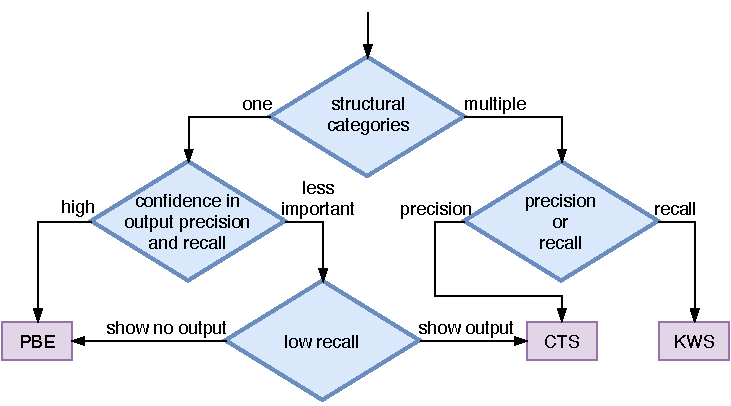
\includegraphics[width=\columnwidth, clip]{img/crt-recommendation.pdf}
		\caption{Our preliminary recommendation scheme for chunk retrieval techniques.}
		\label{fig:crt-recommendation}
\end{figure}

\subsection{Recommendation of Suitable Techniques}
After discussing the three chunk retrieval techniques separately we
now want to unify our results into one recommendation scheme. In
Figure~\ref{fig:crt-recommendation}, we present a decision tree, which
developers and researchers who want to retrieve information chunks
from build logs can follow. The decision tree is built up of questions
which either lead to more questions or to a leaf node containing a
recommended technique. 

\noindent
\textbf{Caveat!} This is a preliminary hypothesis based on the results
from our comparison study. The recommendations could therefore be
influenced by idiosyncrazies of our specific implementation of the
chunk retrieval techniques as well as the logs in the \emph{LogChunks}
data set.

This decision tree in \Cref{fig:crt-recommendation} gives a nunanced
answer to RQ2, about which criteria influence the suitability of a
chunk retrieval technique. The earlier in the decision tree a
criterion is noted, the more important it is when distinguishing the
techniques.

The first and most important aspect are the structural categories. Are
the information chunks one would like to retrieve always presented in
the same structural way within the build logs? Then the information
chunks in all training examples and the analyzed build log are in the
same structural category.

If the information chunks are from multiple structural categories,
i.e. they are not represented in the same structural way within the
build logs, and recall is more important than precision we recommend
to use KWS\@. If the representations are from multiple structural
categories and precision is more important than recall to the user we
recommend CTS\@. We also recommend CTS when the representations are
from one structural category, when the user does not require a high
confidence in the precision or recall of the outcome and when the user
would rather have output with low recall instead of no output at all.
When the representations are from one structural category and the user
wishes a high confidence in the correctness of the output or prefers
no output over output with low recall, we recommend PBE\@.

As a final recommendation, one could create a ``super analyzer'' by
combining the different build log analysis techniques studied in this
paper. Such a super analyzer would likely always first employ PBE
(because of its high accuracy), followed by a combination of CTS and
KWS. Other than initial setup and training time, there should be no
downside to this approach if it is implemented in a transparent way to
the underlying technique: the output of the super analyzer could
include from which sub-tool it originated and thus facilitate
automatic on-ward processing or interpretation of the result.


\noindent
\textbf{Example of Using the Recommendation Scheme}
To illustrate how one would use our decision tree to find a suitable
chunk retrieval technique we describe two concrete examples: a
researcher investigating why CI builds fail and a software team
wanting to monitor their build performance.

In our first example, a researcher studies whether test failures in CI
are caused by a small or by a large group of test cases. They gather
CI build logs from various projects, which are their only available
data source. The task of the researcher is to extract the names of the
failing test cases from each build log. When they use our
recommendation scheme to select a chunk retrieval technique, they
first have to estimate how uniform the representation of the failing
test cases is in the investigated build logs. As the researcher is
covering a wide range of build tools and development languages, the
log chunks they target are in various, non-predictable structural
representations. The next question is whether they value precision
over recall. As they have to manually inspect the results of both CTS
and KWS, they choose recall over precision to avoid having to inspect
the whole log in case the relevant information chunk was not
retrieved. Therefore, our decision tree recommends them to use KWS\@.

In case the researcher wants to avoid manually inspecting the
retrieval results, they have to first separate the CI build logs
according to the test tool responsible for logging the test results.
Then the targeted log chunks are from one structural category and they
can use PBE, trained with examples from each test tool separately.

In our second example, a software development team wants to monitor
the performance of the phases within their CI build. They are using
Travis CI, which measures the duration of build phases and documents
them within the build log. As all log statements that report timing
measurements are formatted the same way, the targeted log chunks are
from one structural category. Therefore the development team can use
PBE to retrieve the duration of a build phase as well as its name.
